\begin{figure}[h] 
\centering 
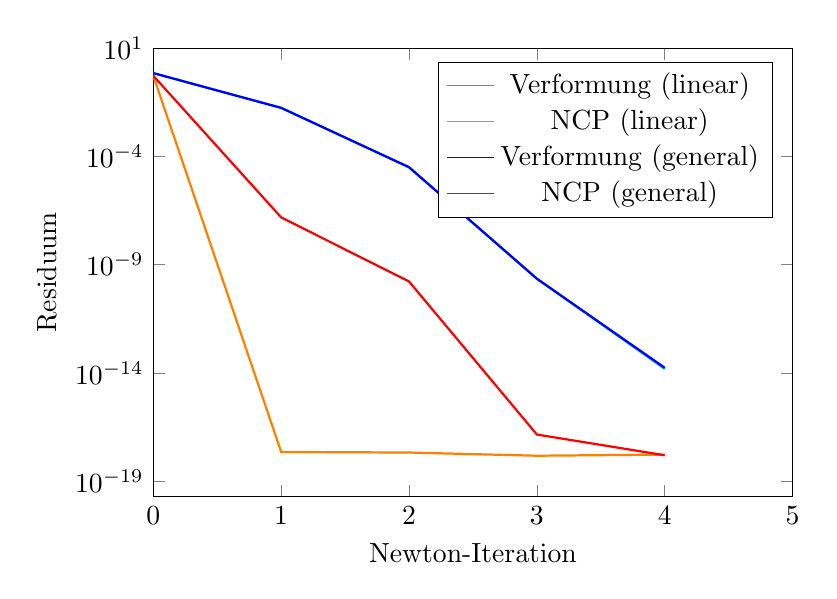
\begin{tikzpicture}[every plot/.append style={thick}] 
\begin{axis}[ 
label style={font=\normalsize}, 
xlabel={Newton-Iteration}, 
ylabel={Residuum}, 
xmin=0, xmax=5, 
ymode=log, 
ymin=0, ymax=10, 
width=0.8\textwidth, 
height=0.6\textwidth, 
legend pos=north east, 
legend style={cells={align=left}}, 
grid style=dashed, 
] 
\addplot[ 
color=cyan, 
] 
coordinates { 
(0, 7.04e-01)(1, 1.75e-02)(2, 3.17e-05)(3, 2.25e-10)(4, 1.56e-14)}; 
\addlegendentry{Verformung (linear)} 
\addplot[ 
color=orange, 
] 
coordinates { 
(0, 5.28e-01)(1, 2.26e-18)(2, 2.12e-18)(3, 1.51e-18)(4, 1.70e-18)}; 
\addlegendentry{NCP (linear)} 
\addplot[ 
color=blue, 
] 
coordinates { 
(0, 7.04e-01)(1, 1.75e-02)(2, 3.18e-05)(3, 2.26e-10)(4, 1.74e-14)}; 
\addlegendentry{Verformung (general)} 
\addplot[ 
color=red, 
] 
coordinates { 
(0, 5.31e-01)(1, 1.53e-07)(2, 1.68e-10)(3, 1.44e-17)(4, 1.59e-18)}; 
\addlegendentry{NCP (general)} 
\end{axis} 
\end{tikzpicture} 
\caption{Residuen des Stoffgesetzes 'Neo Hooke' mit Hinderniss 'Parabel' und 2178 Freiheitsgraden für die Verschiebung.} 
\label{fiq:NeoHooke_Parabel_level4} 
\end{figure} 
